  %  \nonstopmode
\documentclass[10pt,letterpaper,cm]{nupset}
\usepackage[margin=1in]{geometry}
\usepackage{graphicx}
\usepackage{enumerate}
\usepackage{enumitem}
\usepackage{float}
\usepackage{stmaryrd}
\usepackage{amsfonts}
\usepackage{amssymb}
\usepackage{mathtools}
\usepackage{upgreek}
\usepackage{pgfplots}
\pgfplotsset{compat=1.13}
\usepackage{amsmath,amsthm}
\usepackage{tikz-cd}
\usetikzlibrary{backgrounds,calc,positioning}
\usetikzlibrary{knots,calc}
\usepackage{xcolor}
\usepackage{soul}
\usetikzlibrary{decorations.markings}
\usepackage{faktor}
\usepackage{xfrac}
\usepackage{textcomp}
\usepackage{ mathrsfs }
\usepackage{hyperref}
\hypersetup{colorlinks=true, linkcolor=red,          % color of internal links (change box color with linkbordercolor)
    citecolor=green,        % color of links to bibliography
    filecolor=magenta,      % color of file links
    urlcolor=cyan           }
\usepackage{adjustbox}
\usepackage{media9}


\usepackage{thmtools}
\usepackage[capitalise]{cleveref} 
    
\theoremstyle{definition}
\newtheorem{defn}{Definition}[subsection]
\newtheorem{exmp}[defn]{Example}
\newtheorem{non-exmp}[defn]{Non-example}
\newtheorem{note}[defn]{Note}

\theoremstyle{theorem}
\newtheorem{theorem}[defn]{Theorem}
\newtheorem{lemma}[defn]{Lemma}
\newtheorem{prop}[defn]{Proposition}
\newtheorem{fact}[defn]{Fact}
\newtheorem{corollary}[defn]{Corollary}
\newtheorem*{claim}{Claim}
\newtheorem{exercise}[defn]{Exercise}
\newtheorem{conj}[defn]{Conjecture}

\theoremstyle{remark}
\newtheorem{remark}[defn]{Remark}
\newtheorem*{todo}{To do}
\newtheorem*{question}{Question}
\newtheorem*{conv}{Convention}
\newtheorem*{aside}{Aside}
\newtheorem*{notation}{Notation}
\newtheorem*{term}{Terminology}
\newtheorem*{background}{Background}
\newtheorem*{further}{Further reading}
\newtheorem*{sources}{Sources}

\makeatletter
\def\th@plain{%
  \thm@notefont{}% same as heading font
  \itshape % body font
}
\def\th@definition{%
  \thm@notefont{}% same as heading font
  \normalfont % body font
}
\makeatother


\makeatletter
\renewcommand*\env@matrix[1][*\c@MaxMatrixCols c]{%
  \hskip -\arraycolsep
  \let\@ifnextchar\new@ifnextchar
  \array{#1}}
\makeatother
\pgfplotsset{unit circle/.style={width=4cm,height=4cm,axis lines=middle,xtick=\empty,ytick=\empty,axis equal,enlargelimits,xmax=1,ymax=1,xmin=-1,ymin=-1,domain=0:pi/2}}
\DeclareMathOperator{\Ima}{Im}
\newcommand{\A}{\mathcal A}
\newcommand{\C}{\mathbb C}
\newcommand{\E}{\vec E}
\newcommand{\CP}{\mathbb{CP}}
\newcommand{\F}{\mathbb F}
\newcommand{\G}{\frak{G}}
\newcommand{\J}{\mathcal J}
\renewcommand{\H}{\mathbb H}
\newcommand{\HP}{\mathbb HP}
\newcommand{\K}{\mathbb K}
\renewcommand{\L}{\mathcal L}
\newcommand{\N}{\mathbb N}
\renewcommand{\O}{\mathcal O}
\newcommand{\OP}{\mathbb OP}
\renewcommand{\P}{\mathbb P}
\newcommand{\Q}{\mathbb Q}
\newcommand{\I}{\mathbb I}
\newcommand{\R}{\mathbb{R}}
\newcommand{\RP}{\mathbb{RP}}
\renewcommand{\S}{\mathbb S}
\newcommand{\T}{\mathcal T}
\newcommand{\X}{\mathscr X}
\newcommand{\Z}{\mathbb Z}
\newcommand{\B}{\mathbb{B}}
\newcommand{\imp}{\mathsf{Imp}}
\newcommand{\1}{\mathbb{1}}
\newcommand{\ds}{\displaystyle}
\newcommand{\ran}{\right>}
\newcommand{\lan}{\left<}
\newcommand{\bmat}[1]{\begin{bmatrix} #1 \end{bmatrix}}
\renewcommand{\a}{\vec{a}}
\renewcommand{\b}{\vec b}
\renewcommand{\c}{\vec c}
\renewcommand{\d}{\vec d}
\newcommand{\e}{\vec e}
\newcommand{\h}{\vec h}
\newcommand{\f}{\vec f}
\newcommand{\g}{\vec g}
\renewcommand{\i}{\vec i}
\renewcommand{\j}{\vec j}
\renewcommand{\k}{\vec k}
\newcommand{\n}{\vec n}
\newcommand{\p}{\vec p}
\newcommand{\q}{\vec q}
\renewcommand{\r}{\vec r}
\newcommand{\s}{\vec s}
\renewcommand{\t}{\vec t}
\renewcommand{\u}{\vec u}
\newcommand{\w}{\vec w}
\newcommand{\x}{\vec x}
\newcommand{\y}{\vec y}
\newcommand{\z}{\vec z}
\newcommand{\0}{\vec 0}
\newcommand{\pt}{\mathsf{pt}}
\newcommand{\from}{\longleftarrow}
\newcommand{\intprodl}{%
    \mathbin{\scalebox{1.5}{$\lrcorner$}}%
}
\newcommand{\intprodr}{%
    \mathbin{\scalebox{1.5}{$\llcorner$}}%
}

\DeclareMathOperator*{\Span}{span}
\DeclareMathOperator{\rng}{range}
\DeclareMathOperator{\gemu}{gemu}
\DeclareMathOperator{\almu}{almu}
\DeclareMathOperator{\id}{id}
\DeclareMathOperator{\tr}{tr}
\DeclareMathOperator{\vd}{vd}
\DeclareMathOperator{\tor}{Tor}
\DeclareMathOperator{\im}{im}
\DeclareMathOperator{\Sp}{Sp}
\DeclareMathOperator{\codim}{codim}
\DeclareMathOperator{\homeo}{Homeo}
\DeclareMathOperator{\GL}{GL}
\DeclareMathOperator{\SL}{SL}
\DeclareMathOperator{\Or}{O}
\DeclareMathOperator{\SO}{SO}
\DeclareMathOperator{\norm}{N}
\DeclareMathOperator{\aut}{Aut}
\DeclareMathOperator{\Int}{Int}
\DeclareMathOperator{\U}{U}
\DeclareMathOperator{\ext}{Ext}
\DeclareMathOperator{\M}{M}
\DeclareMathOperator{\pic}{Pic}
\DeclareMathOperator{\supp}{supp}
\DeclareMathOperator{\cl}{cl}
\DeclareMathOperator{\dom}{dom}
\DeclareMathOperator{\rnk}{rank}
\DeclareMathOperator{\Hom}{Hom}
\DeclareMathOperator{\Alt}{Alt}
\DeclareMathOperator{\dr}{dR}
\DeclareMathOperator{\ed}{End}
\DeclareMathOperator{\BM}{BM}
\DeclareMathOperator{\ob}{ob}
\DeclareMathOperator{\pgl}{PGL}
\DeclareMathOperator{\clength}{cup{-}length}
\DeclareMathOperator{\sgn}{sgn}
\DeclareMathOperator{\orb}{Orb}
\DeclareMathOperator{\cyl}{Cyl}
\DeclareMathOperator{\rel}{rel}
\DeclareMathOperator{\cat}{cat}
\DeclareMathOperator{\op}{op}
\DeclareMathOperator{\Gd}{Gd}
\DeclareMathOperator{\coker}{coker}
\DeclareMathOperator{\map}{Map}
\DeclareMathOperator{\sing}{Sing}
\DeclareMathOperator{\Op}{\mathbf{Op}}
\DeclareMathOperator{\colim}{colim}
\DeclareMathOperator{\tot}{Tot}
\DeclareMathOperator{\ev}{eval}
\DeclareMathOperator{\sym}{Sym}
\DeclareMathOperator{\BL}{\mathcal{BL}}
\DeclareMathOperator{\bl}{\mathrm{Bl}}
\DeclareMathOperator{\Et}{\acute{E}t}
\DeclareMathOperator{\ch}{\mathbf{Ch}}
\DeclareMathOperator{\vf}{\mathscr{X}}

\newcommand{\vertneq}{\rotatebox{90}{$\,\neq$}}
\newcommand{\net}[2]{\underset{\scriptstyle\overset{\mkern4mu\vertneq}{#2}}{#1}}

\newcommand{\bi}{\begin{itemize}}
\newcommand{\ei}{\end{itemize}}

\newcommand{\be}{\begin{enumerate}}
\newcommand{\ee}{\end{enumerate}}

\newcommand{\bmp}{\begin{mathpar}}
\newcommand{\emp}{\end{mathpar}}

\setlength{\parindent}{0pt}


\newcommand{\bigne}{\text{\scalebox{2}{\ensuremath{\nearrow}}}}

\newcommand{\mathcolorbox}[2]{\colorbox{#1}{$\displaystyle #2$}}

\newlist{steps}{enumerate}{1}
\setlist[steps, 1]{label = Step \arabic*:}

\pagestyle{headings}

\linespread{1.3}

% info for header block in upper right hand corner
\name{Perry Hart}
\class{MATH 622}
\assignment{Fall 2019}

\begin{document}
\thispagestyle{empty}
\begin{abstract}
These notes are based on Ron Donagi's lectures for the course ``Complex Algebraic Geometry'' at UPenn along with Daniel Huybrechts's \textit{Complex Geometry}. Any mistake in what follows is my own.
\end{abstract}

\tableofcontents
\newpage

\section{A cursory overview of algebraic geometry} 

\subsection{Lectures 1-4}

These lectures consisted of informal surveys of certain fundamental concepts of algebraic geometry. They were meant as previews of various topics that we will cover rigorously. The following three problems give a taste of the initial concepts presented.

\medskip

\begin{problem}[Projective space.]

Recall that projective space $\P^n$ of dimension $n$ is by definition the	quotient	of $\mathbb{A}^{n+1}\setminus \left\{0\right\}$		by	the	rescaling	action	of	$\GL(1)$.	This 	is a compactification	of	$n$-dimensional affine	space	$\mathbb{A}^n$.
Show	that	$\P^n$	has	an	open	covering	by	$n+1$ many	open	subsets	$U_0,\ldots,U_n$	each	isomorphic	to $\mathbb{A}^n$.	Work	 out	all of the	transition	functions.
\end{problem}
\begin{solution}
For simplicity, assume that $\mathbb{A}^n = \mathbb{R}^n$.  For each $i \in \left\{ 1, \ldots, n+1\right\}$, let $\widetilde{U_i}= \left\{\x \in \R^{n+1} : x_i \ne 0\right\}$. Let $\pi: \R^{n+1} \setminus \left\{0\right\} \twoheadrightarrow \RP^n$ denote the natural projection and let $U_i = \pi\left(\widetilde{U_i}\right)$. Since $\widetilde{U_i}$ is saturated and open, we know that $\pi \restriction_{\widetilde{U_i}}$ is a quotient map. Define $f_i : U_i \to \R^n$ by $\left[x_1, \ldots, x_{n+1}\right] \mapsto \left(\frac{x_1}{x_i}, \ldots, \frac{x^{i-1}}{x_i}, \frac{x^{i+1}}{x_i}, \ldots \frac{x_{n+1}}{x_i}\right)$, whose inverse is given by  $\left(x_1, \ldots, x_n\right) \mapsto \left[x_1, \ldots, x_{i-1}, 1, x_{i+1}, \ldots x_n\right]$. Since $f_i \circ \pi$ is continuous, so is $f_i$. Hence we see that $f_i$ is a homeomorphism. 

\smallskip

Now, consider any transition map $f_i \circ f_j^{-1}$. 
Let $1\leq i,j\leq n+1$. If $i=j$, then the transition map is the identity, which is smooth. So assume, wlog, that $j< i$.  Then $$f_j \circ f_i^{-1}(x_1, \ldots, x_n) = \left(\frac{x_1}{x_{j}}, \ldots, \frac{x_{j-1}}{x_{j}}, \frac{x_{j+1}}{x_{j}}, \ldots, \frac{x_{i-1}}{x_{j}}, \frac{1}{x_j}, \frac{x_{i}}{x_{j}}, \ldots, \frac{x_{n}}{x_{j}}\right)$$ when $\left(x_1, \ldots, x_n\right) \in f_i\left(\widetilde{U}_i \cap \widetilde{U}_j\right)$. This is clearly smooth. 
\end{solution}

\begin{problem}[Classification	of	conics.]

Classify, up to linear automorphism, all conics	(i.e., $1$-dimensional	quadratic
hypersurfaces)	in	$\RP^2$.
\end{problem}
\begin{solution}
First of all, we may assume that any conic $C(x,y,z) =0$ in $\RP^2$ is a homogeneous polynomial of degree two. As a result, we can write  $C(x,y,z)= v^tAv$  for some symmetric $3\times 3$ matrix $A$ over $\R$ where $$v \coloneqq \begin{bmatrix} x \\ y \\ z \end{bmatrix}.$$  Since $A$ is orthogonally diagonalizable, we have that $C(v) = \left(Tv\right)^tD(Tv)$ for some orthogonal matrix $T$ and some diagonal matrix $D$.  Thus, $C$ is isomorphic to a curve in $\RP^2$ defined by $0 = a_1x^2 + a_2y^2 + a_3z^3$. We can apply another invertible change of variables to ensure that $a_i \in \left\{{-1}, 0, 1\right\}$ for each $i=1,2,3$.

\smallskip

Likewise, any quadratic hypersurface in $\CP^n$ is isomorphic to a curve in $\CP^n$ defined by $\sum_{i=1}^{n+1}a_ix_i^2 = 0$ where $a_i \in \left\{{-1}, 0, 1\right\}$ for each $i=1, \ldots, n+1$.

\medskip

We now see that there are exactly five distinct automorphism classes of conics in $\RP^2$:
\be[label=(\alph*)]
\item $\left[x^2 =0\right]$ (a double line),
\item $\left[x^2 + y^2 =0\right]$ (a single point),
\item $\left[x^2 -y^2= \left(x-y\right)\left(x+y\right)=0\right]$ (the union of two distinct lines that intersect at a single point),
\item $\left[x^2 +y^2 + z^2 =0\right]$ (the empty set), and
\item $\left[x^2 + y^2-z^2 =0\right]$ (a curve $C$ whose affine part is either an ellipse, a parabola, or a hyperbola, depending on whether $C$ intersects the line at infinity at zero, one, or two points, respectively).
\ee

\end{solution}

\begin{problem}[Plane cubics.]

Recall that a plane curve $C$ is \textit{smooth} if it has no \textit{singular} points, i.e., points at which all first-order partial derivatives of $C$ vanish.
\be
\item Consider	a	smooth	plane	cubic	 $X$	with	an	inflection	point, i.e., a non-singular point at which the tangent line to $X$ has
intersection multiplicity at least $3$ with $X$. Show that $X$	is	isomorphic,	up	to	linear	automorphism	of	the	ambient	space,		to	a
smooth	plane	cubic 	in	\textit{Weierstrass	form} $y^2 = x^3+ax+b$.
\item 	Find	a	an	expression	of	the	form	$J\coloneqq \frac{a^m}{b^n}$	for	some	integers	$m$ and $n$	that	is	invariant	under	linear	changes	of	coordinates 	sending
our	equation	of	$X$	to	another	Weierstrass	form.
\item 	A	slight	 problem	with	$J$	is	that	it	goes 	to	infinity	when	$b=0$	even	 though	the	plane	cubic 	$X$	remains	smooth.	Can	you	suggest
another	function	$j(a,b)$	which	has	the	same	invariance	property as $J$	 but	remains		finite	(i.e.	is	holomorphic)	whenever	$X$	is	smooth?
Relate	$j$	to	$J$.
\ee
\end{problem}
\begin{solution}
\be
\item Any linear automorphism of $\C^3$ induces a projective transformation of $\CP^2$ (i.e., an element of $\pgl(3, \C)$), and the group of all linear automorphisms of $\C^3$ acts transitively on the set of all $2$-dimensional subspaces of $\C^3$. It follows that for any two lines $L_1, L_2 \subset \CP^2$, there is some projective transformation $\psi : \CP^2 \to \CP^2$ such that $\psi(L_1) = L_2$. In particular, we can assume that the tangent line $L$ to our given inflection point $P$ is precisely the line at infinity $\left\{z=0\right\}$ and that any other line touching $P$ is precisely the line $\left\{x=0\right\}$. This means that $P$ corresponds to the point $\left[0, 1, 0\right]$ on our new, isomorphic copy $X'$ of $X$. Note that $X'$ is smooth since any projective transformation preserves smoothness by the familiar multivariable chain rule.

Let $X'$ be the zero locus of the homogeneous polynomial $f(x,y, z)$ of degree three. This has the form $$ Ax^3 + Bxy^2 + Cyx^2 + Dy^3 +zg(x,yz)     $$ where $g(x,y,z)$ denotes a homogenous polynomial of degree two. We have that $d =0$ because $\left[0,1,0\right]$ lies on $X'$. Further, we have that $b=c=0$ because $\left\{z=0\right\}$ is tangent to an inflection point. Therefore, the affine part of $X'$ has the form $$f(x, y,1) =  Ax^3 + Bx^2  + Cxy + Dy^2+ Ex + Fy + G  $$ where both $A$ and $D$ are nonzero. By scaling this appropriately, we may write $$f(x, y,1) = x^3 + Bx^2 + Cxy - y^2 + Ex + Fy + G$$ for some $B, C, E, F, G \in \C$. 

It remains to show that there exists an invertible affine map (or change or variables) $\C^2 \to \C^2$ that sends the zero locus of $f(x,y,1)$ to the zero locus of a cubic polynomial in Weierstrass form. To this end, first define the mapping $f : \left(x,y\right) \mapsto \left(x, \frac{ y+Cx+F }{2}\right)$. A tedious computation shows that $\varphi$ transforms the affine part of $X'$ to the curve $X''$ given by $ \frac{y^2 -F^2- C^2x^2}{4} - \frac{CFx}{2} = x^3 + Bx^2 + Ex + G    ,$ i.e., $$y^2 = 4x^3 + (C^2  + 4B)x^2 + (4E +2CF)x + (4G + F^2).$$ Substituting $2y$ for $y$, we can write $X''$ as $$ y^2 = x^3 + \left(\underbrace{\frac{C^2}{4}  + B}_{k_1} \right)x^2 + \left(\underbrace{E+ \frac{CF}{2}}_{k_2} \right)x + \left(\underbrace{G + \frac{F^2}{4}}_{k_3} \right)   .$$ Next, define the mapping $g : \left(x,y\right) \mapsto \left(x- \frac{k_1}{3}, y\right)$. By another tedious computation, we see that $g$ sends $X''$ to the curve given by $$ y^2 = x^3 + \left (k_2- \frac{\left(k_1\right)^2}{3} \right )x + \left (k_3 + \frac{2\left(k_1\right)^3}{27}- \frac{k_1k_2}{3} \right)    .$$ Since $f$ and $g$ are invertible affine maps, we are done. 
\item Note that any linear change of variables preserving Weierstrass form must look like $\left(x,y\right) \mapsto \left(r^2x, r^3y\right)$ with $r \ne 0$. Let $J = \frac{A^3}{B^2}$. It's straightforward to check that $J$ is invariant under any affine map of the form $\left(x,y\right) \mapsto \left(r^2x, r^3y\right)$.
\item Let $j = \left(27\right)\left(4^4\right)\left(\frac{A^3}{4A^3 + 27B^2}\right).$ This quantity is well-known as the \textit{j-invariant}. Though tedious,  checking that $j$ is invariant under any suitable linear change of variables is still straightforward. In addition, elementary algebra shows that $J = \frac{j}{(27)(4^4)} + \frac{A^3\left(4A^3 + 26B^2\right)}{B^2\left(4A^3 + 27B^2\right)}$.
\ee

\end{solution}

\section{Complex analysis}

\subsection{Lecture 5}

First, let's review some basic concepts about functions of a single complex variable.

\begin{defn}
Let $z_0\in \C$. A function $f = u+iv : U\subset \C \to \C$ is \textit{holomorphic} or \textit{analytic} if at least one of  the following equivalent conditions holds.
\be[label=(\roman*)]
\item Both $u$ and $v$ are $C^1$, and $f$ satisfies the Cauchy-Riemann equations, i.e., 
\begin{align*}
u_x & = v_y
\\ u_y & = {-v_x}.
\end{align*}
\item $\frac{\partial{f}}{\partial{\bar{z}}} =0$, where $\frac{\partial}{\partial{\bar{z}}} \coloneqq \frac{1}{2}\left(\frac{\partial}{\partial{x}} + i\frac{\partial}{\partial{y}}\right ) .$
\item The Cauchy integral formula holds, i.e., 
\[f(w) = \frac{1}{2\pi i}\int_{\gamma}\frac{f(w)}{\eta -w}d{\eta}
\] for any closed circular path $\gamma$ centered at $w$ in $U$. 
\item $f$ has a power series representation on $U$.
\ee
\end{defn}

\smallskip

\begin{defn}
A bijective function $f: U \subset \C \to V \subset \C$ is \textit{biholomorphic} if it is holomorphic and its inverse is holomorphic. In this case, we say that $U$ is \textit{biholomorphic to} $V$, written as $U \approx V$.
\end{defn}

\begin{fact}\label{singfacts} $ $
\be[label = (\alph*)]
\item{\textbf{Maximum modulus principle.}} If $U\subset \C$ is a domain, $f: U \to \C$ is holomorphic, and $\left\lvert{f}\right\rvert$ has a local maximum, then $f$ is constant. 
\item{\textbf{Liouville's theorem.}} Any bounded entire function is constant. 
\item{\textbf{Riemann extension theorem.}} If $\epsilon >0$ and $f: B_{\epsilon}(z) \setminus \left\{z\right\} \subset \C \to \C$ is bounded and holomorphic, then $f$ can be extended to a holomorphic function on $B_{\epsilon}(z)$.
\item{\textbf{Riemann mapping theorem.}} If $U\subsetneq \C$ is simply connected and open, then $U\approx B_1(0)$. 
\item{\textbf{Residue theorem.}} If $f: B_{\epsilon}(0)\setminus \left\{0\right\}$ is holomorphic, then $f$ can be expanded in a Laurent series
$\sum_{n={-\infty}}^{\infty}a_nz^n$ such that $a_{-1} = \frac{1}{2\pi i}\oint f(z)d{z}$.
\ee
\end{fact}

\medskip

Next, let's look at some basic concepts about functions of several complex variables.

\begin{defn}
A function $f = u +iv: U\subset \C^n \to \C$ is \textit{holomorphic} if at least one of  the following equivalent conditions holds.
\be[label=(\roman*)]
\item $f$ is holomorphic in each variable individually.
\item  Both $u$ and $v$ are $C^1$, and $f$ satisfies the Cauchy-Riemann equations,
\begin{gather*}
u_{x_i}  = v_{y_i}
\\ u_{y_i}  = {-v_{x_i}}
\end{gather*}
for each $i=1, \ldots, n$.
\item $\sum_{i=1}^n\frac{\partial{f}}{\partial{\bar{z}_i}} =0$.
\item $f$ has a power series representation on $U$,
\[
\sum_{k_1=0}^{\infty}\cdots \sum_{k_n=0}^{\infty} a_{k_1, \ldots, k_n}z_1^{k_1}\cdots z_n^{k_n}.
\]
\ee
\end{defn}

\begin{note}
Statements (a), (b), and (c) of \cref{singfacts} generalize to functions of several variables, as does the Cauchy integral formula:
\[
f(z) = \frac{1}{(2\pi i)^n} \int_{\left\lvert{\eta_i - z_i}\right\rvert = \epsilon_i} \frac{f(\eta_1, \ldots, \eta_n)}{\left(\eta_1 - z_1\right)\cdots \left(\eta_n - z_n\right)}d{\eta_1}\cdots d{\eta_n}
\] where $\eta_i >0$ for each $i=1, \ldots, n$.
\end{note}

\begin{theorem}[Hartog]
If $n>1$, then any holomorphic function $f: B_{\epsilon}(0)\setminus \left\{0\right\} \subset \C^n \to \C$ extends to a holomorphic function on $B_{\epsilon}(0)$.
\end{theorem}

\begin{defn} Let $X$ be a (topological) space. A \text{sheaf $F$ on $X$} is a presheaf on $X$ such that for any open $U\subset X$ and any open cover $\left\{U_i\right\}_{i\in J}$ of $U$, there is an exact sequence
\[
\begin{tikzcd}
0 \arrow[r] & F(U) \arrow[r] & F(U_i) \arrow[r] & F(U_{ij})
\end{tikzcd}
\] where $U_{ij} \coloneqq U_i \cap U_j$.
\end{defn}

\begin{exmp}
Let $S$ be a suitable object (such as a set or $R$-module)  and $x\in X$. The \textit{skyscraper sheaf} of $X$ supported at $x$ with value $S$ is given by
\[
\left(\underset{\text{open}}{U \subset X}\right) \mapsto \begin{cases}
S & x\in U
\\ \pt & x\notin U
\end{cases}.
\]
\end{exmp}

\smallskip

\begin{defn}
A \textit{ringed space} is a pair $\left(X, \J\right)$ where $X$ is a space and $\J$ is a sheaf of rings on $X$.
\end{defn}

\begin{remark} Given any standard object $\left(X, \J\right)$, we can define a \textit{geometric object} as a ringed space locally isomorphic to $\left(X, \J\right)$.
\end{remark}

\medskip

\begin{defn}[Vector bundle]
Let $X$ and $V$ be complex manifolds. Let $\pi : V \to X$ be holomorphic. We say that $\pi$ is a \textit{(holomorphic) vector bundle of rank $n$} if for any $x\in X$, there exist an open set $U\ni x$ in $X$ and an isomorphism $\pi^{-1}(U) \overset{\cong}{\longrightarrow} U \times \C^n$ such that the \textit{transition maps} $U_{ij} \times \C^n \to U_{ij} \times \C^n$ are holomorphic and fiber linear.
\end{defn}

\smallskip

Any vector bundle $\pi : V \to X$ induces a sheaf on $X$ given by
\[
F(U) = \Gamma\left(U, \pi^{-1}(U)\right).
\]

\begin{exmp} $ $
\be
\item The sheaf induced by the trivial bundle $\mathbf{1} \coloneqq X \times \C$ is denoted by $\O_X$.
\item The tangent bundle $T{X}$ of a smooth manifold $X$ induces the sheaf of vector fields on $X$.
\item The cotangent bundle $T^{\ast}{X}$ induces the sheaf $\Omega^1(X)$ of one-forms on $X$.
\item The alternating bundle $\bigwedge^p{X}$ of rank $p$ induces the sheaf $\Omega^p(X)$ of $p$-forms on $X$.
\ee
\end{exmp}

\section{Line bundles}

\subsection{Lecture 6}

\begin{defn}
A \textit{line bundle} is a vector bundle of rank $1$.
\end{defn}

\begin{defn}
Let $X$ be a complex manifold.  A \textit{sheaf $F$ of $\O_X$-modules} is a sheaf on $X$ such that for any open set $U$ in $X$,
\be[label=(\roman*)]
\item $F(U)$ is a module over $\O_X(U)$ and
\item if $U \subset V \subset X$, then $\left(f\cdot a\right)\restriction_U = f\restriction_U\cdot a\restriction_U$.
\ee
\end{defn}

\begin{exmp}[Sheaf of sections]
Let $X$ be a complex manifold and $J$ be a vector bundle over $X$. For any open $U\subset X$, let $$\L_J(U) = \Gamma\left(U, L\right).$$ This inherits a vector space structure from the family of fibers of $V$. Also, any relation of the form $U_1 \subset U_2 \subset U$ induces a linear map $\Gamma\left(U_2, L\right) \to \Gamma\left(U_1, L\right)$ given by $\sigma \mapsto \sigma\restriction_{U_1}$. Thus, $\L_J\left({-}\right)$ is a sheaf of vector spaces. Moreover, it is easily seen to be a sheaf of $\O_X$-modules. 
\end{exmp}

Since any vector bundle is locally trivial, we see that $\L_J$ is \textit{locally free}, i.e., for any $x\in X$, there exist an (open) neighborhood $U$ of $x$ in $X$ and an isomorphism $\varphi : \L_J(U) \to \bigoplus_{i=1}^{\rnk(J)}\O_X(U)$ such that for any open set $V\subset U$, the square
\[
\begin{tikzcd}
\L_J(U) \arrow[r, "\cong"] \arrow[d] &  \bigoplus_{i=1}^{\rnk(J)}{\O_X(U)} \arrow[d] \\
\L_J(V) \arrow[r, "\cong"']          &  \bigoplus_{i=1}^{\rnk(J)}{\O_X(V)}          
\end{tikzcd}
\]
commutes. In other words, $\L_J$ is locally isomorphic to $\left(\O_X\right)^{\oplus{\rnk(J)}}$.

\begin{defn} 
A sheaf $F$ on a complex manifold $X$ is \textit{invertible} if there exist an open cover $\left\{U_i\right\}$ of $X$ and a family of holomorphic isomorphisms $\varphi_i : \O_{U_i} \to \L_J\restriction_{U_i}$.
\end{defn}

\begin{exmp} 
If $J$ is a line bundle, then $\L_J$ is invertible.
\end{exmp}

Consider the composite
\[
\begin{tikzcd}
\O_{U_i \cap U_j} \arrow[r, "\varphi_i"] & \L_J\restriction_{U_i \cap U_j} \arrow[r, "\varphi_j^{-1}"] & \O_{U_i \cap U_j}
\end{tikzcd}
, \ \quad \quad 1 \longmapsto g_{ij}.
\] From this, we can construct a line bundle $L$ over $X$ by defining the total space as 
\[
\faktor{\coprod_i\left(U_i \times \C\right)}{\sim}
\] where $\left(x, \lambda \right)_i \sim \left(y, \mu\right)$ if $x=y$ and $\mu = g_{ij}\lambda$. 

\medskip

\begin{defn}[Divisor]
A \textit{divisor on a complex manifold $X$} is a locally finite $\Z$-combination of irreducible holomorphic hypersurfaces of $X$. Equivalently, it is a subset of $X$ locally defined  by the vanishing of a holomorphic function.
\end{defn}

\begin{exmp}
If $X = \A^1$, then any divisor $D$ on $X$ is of the form $$D = \sum m_ip_i, \ \quad p_i \in \A^1, \ m_i \in \Z.$$ 
\end{exmp}

\begin{term}
Each $m_i$ is known as the \textit{multiplicity of $p_i$}.
\end{term}

Any divisor $D$ defines a line bundle $\O_X(D)$ on $X$ and a holomorphic map $X \dashrightarrow \P\left(V^{\vee}\right)$ where $V\equiv \Gamma\left(X, \O_X(D)\right)$. It is also true that any line bundle defines a divisor. It follows that
\[
\begin{tikzcd} 
\label{eqn:corr}
\left(\text{line bundles}\right) \arrow[r] & \left(\text{invertible sheaves}\right) \arrow[l, "\sim"'] \arrow[r] & \left(\text{divisors module linear equiv.}\right) \arrow[l, "\sim"'] \tag{$\dagger$}
\end{tikzcd}.
\]

\medskip

Consider the case where $D = \pt$. Let $f \in \Gamma\left(U, \O_U\right)$ and let $U_i = X \setminus D$, which is a tubular neighborhood of $D$. Note that $U_i = f^{-1}\left (\C\setminus\text{hyperplane}\right)$. Define $\O_X(D)$ as the line bundle with transition functions of the form $f \restriction_{U_i \cap U_j}$.

\medskip

Alternatively, let $$\left(\O_X\left(D\right)\right)\left(U\right) = \left\{g : U \to \C  \mid g \text{ is meromorphic}, \ \overbrace{fg}^{\text{\tiny product}} \text{ is holomorphic}\right\}.$$
For example,
let $X = \P^1$ and $D$ be a point $p$. Let $\left(x_0, x_1\right)$ denote local coordinates on $X$ near $p$. Let $g$ be meromorphic in these coordinates and let $f\left(x_0, x_1\right) = \frac{x_1}{x_0}$. Then $f{g}$ is holomorphic, i.e., $g$ has a pole of order at most one at $p$. 
\begin{question} $ $
\be
\item What is $\Gamma\left(\P^1, \O_X\right)$?
\item What is $\Gamma\left(\P^1, \O_X\left(D\right)\right)$?
\ee
\end{question}

In fact, it can be shown that
\[
\Gamma\left(\P^1, \O_X\left(m,p\right)\right) = \begin{cases}
\C\langle 1, x, \ldots, x^m\rangle & m \geq 0 
\\ 0 & \text{otherwise}
\end{cases}
\]

\bigskip

In general, $D$ is defined locally, and thus so is $\O_U(D)$. Specifically,
$\Gamma\left(U, \O_U\left(D\right)\right)$ consists of all holomorphic functions $f : U \setminus \supp\left(D\right) \to \C$ such that if $D = \sum m_iY_i$ and $Y_i \cap U = \left\{f_i =0\right\}$, then $g\prod_if_i^{m_i}$ is holomorphic in $U$.

\begin{exmp}[Veronese embedding]
Let $X = \P^1$ and $p$ be as before. 
\be
\item Let $D = \O(2p)$. Consider the space $V \coloneqq \Gamma\left(\P^1, \O\left(2p\right)\right) = \C\langle 1, x, x^2\rangle.$ Define the map $\varphi_{\O(2p)} : \P^1 \to \P^2$ by $$\varphi_{\O(2p)}(x) = \underbrace{\left(1, x, x^2\right)}_{\left(x,y,z\right)}.$$ This is an embedding. Its image is precisely the smooth curve given by $y^2 = xz$.
\item Let $D = \O(3p)$. Then the image of the map $\varphi_{\O(3p)} : \P^1 \hookrightarrow \P^3$ given by $x \mapsto \left(1, x, x^2, x^3\right)$ is a so-called twisted cubic.
\ee
\end{exmp}


The line bundle $L$ on $X$ determines the map $X \dashrightarrow \P\left(\Gamma\left(X, L\right)^{\vee}\right)$ directly, as follows.
\[
x\mapsto \ker\left(\Gamma\left(X, L\right) \overset{\ev_x}{\longrightarrow} L_p\right)
\]

\begin{defn}
The \textit{base locus of $L$} is $\BL\left(L\right) \equiv \left\{x  \in X \mid s(x) =0 \text{ for each } s\in \Gamma\left(X, L\right)\right\}$.
\end{defn} 

Note that we get a map $X \setminus \BL\left(L\right) \to \P\left(\Gamma\left(X, L\right)^{\vee}\right)$.

\bigskip

Now, let's consider a slight generalization of our preceding discussion. Let $V \subset \Gamma\left(X, L\right)$. This induces a map 
\[
\begin{tikzcd}
X \arrow[r, dashed]                                    & \P\left(V^{\vee}\right) \\
X\setminus\BL\left(V\right) \arrow[u, hook] \arrow[ru] &                        
\end{tikzcd}.
\]

Let $X = \P^1$ and $p = \left\{x=0\right\}$. Then $V \subset \Gamma\left(\P^1, \O(2)\right) = \C\langle 1, x, x^2\rangle$, and
\[
\begin{tikzcd}
\P^1 \arrow[rd, "\varphi_V"', dashed] \arrow[r, "\varphi_{\O(2)}"] & \P^2 \arrow[d, "\rho", dashed] \\
                                                                   & \P^1                       
\end{tikzcd}
\] commutes where $\rho$ denotes the linear projection. Note that $\varphi_V$ is a morphism so long as the center of $\rho$ is not in the image of $\varphi_{\O(2)}$. In this case, we have that
\begin{align*}
\varphi_{\O(2)}(x) & = \frac{a +by + cx^2}{d + ex +fx^2}
\\  \rho(x) & = \frac{a+bx}{c+dx}.
\end{align*}

\subsection{Lecture 7}

Let $L_1$ and $L_2 $ be line bundles over $X$ with transition functions $\left\{g_1^{k{l}} : U_{k{l}} \to \C^{\ast}\right\}$ and $\left\{g_2^{i{j}} : U_{i{j}} \to \C^{\ast}\right\}$, respectively. We can take a refinement $\left\{U_{i} \cap U_k\right\}$ where both $L_1$ and $L_2$ are trivial.  Define $L^1 \otimes L^2$ as the line bundle with transition functions $\left\{g_1^{k{l}}g_2^{i{j}} : U_{ij} \cap U_{k{l}} \to \C^{\ast}\right\}$. Further, define $\left(L^1\right)^{-1}$ as the line bundle with transition functions $\left\{\left(g_1^{k{l}}\right)^{-1} : U_{k{l}} \to \C^{\ast}\right\}$. Note that, locally, $L^1 \otimes \left(L^1\right)^{-1} \cong \O_X$.

\begin{defn}
We say that a divisor $D = \sum_im_iY_i$ is \text{effective} if $m_i\geq 0$ for each $i$.
\end{defn}

Let $V = \Gamma\left(X, \O_X(D)\right)$ and let $D$ be effective. Note that $\C\langle D \rangle \subset V$. We have that $\supp(D) = \varphi^{-1}\left(\text{hyperplane}\right)$ where $\left(\C \langle 0\rangle \right)^{\perp}$ is precisely the hyperplane in $\P\left(V^{\vee}\right)$.

\begin{exmp} Let $X = \P^1$.
\be
\item Let $x= \frac{x_1}{x_0}$ and $D =p \coloneqq \left\{x=0\right\}$. Then $V = \C\langle 1, x \rangle$, and the map $\varphi_V : \P^1 \to \P\left(V^{\vee}\right)$ is given by $c\mapsto y\coloneqq \frac{x}{1}$.
\item Let $D = m\left(\infty\right)$ with $m>0$. Then $V= \C\langle x_1, \ldots, x_m^m\rangle$, and the map $\varphi_{m{\infty}} : \P^1 \to \P^m$ is given by
\begin{align*}
\left(x_0, x_1\right) & \mapsto \left(x_0^m, x_0^{m-1}x_1, \ldots, x_0x_1^{m-1}, x_1^m\right)
\\ x \ & \mapsto \  \left(1, x, \ldots, x^m\right).
\end{align*}
\item Let $D = p_1 + \cdots + p_m$ where $p_i = \left[1:t_i\right]$. Let $x = \frac{x_1}{x_0}$, so that $\infty$ is given by $x_0 =0$. Then $V = \C\langle \underbrace{1, \frac{1}{x-t_1}, \ldots, \frac{1}{x-t_m}}_{a_0, \frac{a_1}{x-t_1}, \ldots, \frac{a_m}{x-t_m}}\rangle$. This can be viewed as the space of all regular meromorphic functions on open subsets of $\P^1$ having poles of order at most $m$. The image of $\varphi : \P^1 \to \P^m$ is precisely the hyperplane $\left\{a_0 =0\right\}$.
\ee
\end{exmp}

\begin{exmp}
Let $X$ be an elliptic curve, i.e., a space of the form $\C/\Lambda$. Let $p$ be the image of $0$ and let $D = mp$. 
\be
\item Let $m =1$. Then $V = \Gamma\left(X, \O_X(D)\right)$, which consists of all maps $f: X \to \P^1$ such that $f^{-1}\left(\infty\right) = \left\{0\right\}$. These are precisely the constant maps, so that $V \cong \C\langle s\rangle$ where $s$ is a holomorphic section of $\O_X(D)$ vanishing at $p$ and is meromorphic on $\O_X$.
\[
\begin{tikzcd}
X \arrow[r, dashed]                     & \P^0 \\
X\setminus p \arrow[u, hook] \arrow[ru] &     
\end{tikzcd}
\]
It follows that  $\BL\left(\O_X(D)\right) =p$.
\item Let $m=2$. Then $V= \C\langle 1, p\rangle$, and $\varphi_{2p} : X \to \P^1$ is precisely the $D$-th Weierstrass function. Moreover, we have an exact sequence
\[
\begin{tikzcd}
0 \arrow[r] & \O_X(p) \arrow[r] & \O_X(2p) \arrow[r] & \O_p \arrow[r] & \cdots
\end{tikzcd}.
\]
\item Let $m=3$. Then $V = \langle 1, p, p'\rangle$, and the image of $\varphi_{3p} :X \to \P^2$ is given by $y^2 = x^3+ax+b$. 
\ee
\end{exmp}

\begin{exmp} Let $X = \P^2$. Let $D= m\underbrace{\left(\text{line at }\infty\right)}_{\{z=0\}}$.
\be
\item Let $m=0$. Then $V = \C\langle 1\rangle$, and $\BL= \emptyset$.
\item Let $m=1$. Then $C = \C\langle \frac{x}{z}, \frac{y}{z}, \frac{z}{z}\rangle \cong \C\langle 1, X, Y\rangle$, and $\BL = \emptyset$. The map $\varphi_D : \P^2 \to \P^2$ is precisely the identity. 
\item Let $m=2$. Then $V = \langle \frac{x^2}{z^2}, \frac{x^4}{z^2}, \frac{y^2}{z^2}. \frac{x}{z}, \frac{y}{z}, \frac{z}{z}\rangle$, and the map $\varphi_D : \P^2 \to \P^5$ is an embedding given by $\left(x,y,z\right) \mapsto \langle x^2, xy, y^2, xz, yz, z^2\rangle$.
\ee
\end{exmp}

In general, if $H\subset \P^n$ is a hyperplane, then $\varphi_{\O\left(d{H}\right)} : \P^n \to \P^{{{d+n}\choose n} -1}$ is given by $$\left(x_0, \ldots, x_n\right) \mapsto \left(d\text{-th order homogenous polynomials}\right),$$  known as the $d$-th order Veronese embedding on $\P^n$.

\begin{exmp}
Let $X = \P^2$ with coordinates $\left(x,y,z\right)$. Let $H$ denote the hyperplane given by $z=0$ and let $D = 2{H}$. Then $ V= \left\{s\in \Gamma  \left(\O\left(2{H}\right)\right) \mid s\left(0,0,1\right) =0\right\}$, and
\[
\begin{tikzcd}
V \arrow[r, hook]                                                         & \Gamma\left(\O\left(2{H}\right)\right)                           \\
{\C\langle x^2, xy, y^2, xz,yz\rangle} \arrow[r, hook] \arrow[u, "\cong"] & {\C\langle x^2, xy, y^2, xz, yz, z^2\rangle} \arrow[u, "\cong"']
\end{tikzcd}
\] commutes. Further, $\BL(V) = \left\{0\right\} = \left[0,0,1\right]$, and $\varphi_V$ is a map $\P^2 \setminus \left\{0\right\} \to \P^4$ but does not extend to $\P^2$. Indeed, we have that
\begin{align*}
\lim_{\substack{\left(0, y, 1\right) \\ y\to 0}} \varphi_V  & = \lim_{y\to0}\left(0,0,y^2,0, y\right)= \net{\left(0,0,0,0,1\right)}{}
\\ \lim_{\substack{\left(x, 0, 1\right) \\ x\to 0}} \varphi_V  & = \lim_{x\to0}\left(x^2,0,0,x, 0\right)= \left(0,0,0,1,0\right).
\end{align*} Note that for any $p\in X$, there exist $\widetilde{X}$ and $\pi : \widetilde{X}\to X$ such that $\pi$ restricted to $\pi^{-1}\left(X\setminus p\right)$ is an isomorphism and $\pi^{-1}(p)$ is a divisor on $\widetilde{X}$ that is isomorphic to $\P^1$.
\end{exmp}

\begin{prop}
Let $Y \subset X$ be a submanifold of codimension $k\geq 2$. Let $\varphi : X \setminus Y \to Z$. Then there exist $\widetilde{X}$ and $\pi : \widetilde{X}\to X$ such that $\pi$ restricted to $\pi^{-1}\left(X\setminus Y\right)$ is an isomorphism and restricted to $\underbrace{\pi^{-1}(Y)}_{\text{divisor on }X}$ is a bundle with each fiber isomorphic to $\P^{k-1}$.
\end{prop}

\begin{notation}
In this case, the space $\widetilde{X}$ is denoted by $\bl_Y(X)$.
\end{notation}

\subsection{Lecture 8}

Recall our correspondence \eqref{eqn:corr}. We can add to it the class of all maps $$X \setminus \BL(L) \to \P\left(\Gamma \left(X, L\right)^{\vee}\right).$$
Let's turn now to some higher-dimensional examples.

\begin{exmp}
Let $X = \P^2$, $L = \O(2)$, and $V = \left\{s\in \Gamma\left(X, \O(2)\right) \mid \text{linearity condition}\right\}$. Then $\varphi_V : \P^2 \hookrightarrow \P^5$. Consider any homogenous polynomial $\sum a_{ijk}x^iy^jz^k$. Then our linearity condition may take any of the following forms. 
\bi
\item $\sum a_{ijk}x^iy^jz^k =0$ where $a_{ijk}$ ranges over
\[
\{a_{000}, a_{120}, a_{020}, a_{101}, a_{011}, a_{002}\}.
\] 
\item $a_{002}=0$ 
\item $a_{002} +a_{001} =0$.
\ei
In the case of either of these last two, we get a map 
\[ \begin{tikzcd}
\P^2 \arrow[r, "\varphi_V"] & \P^5 \arrow[r, "\psi", dashed] & \P^4
\end{tikzcd}
\] for any $p\in \P^5$. There are two scenarios to consider.
\be[label = (\alph*)]
\item Suppose that $p \notin \im{\varphi_V}$. Then $\psi \circ \varphi_V$ is a morphism.
\item Suppose that $p = \varphi_V\left(001\right)$. Then $\psi$ blows up at $p$. Consider the map $\varphi_V : \P^2\setminus p \hookrightarrow \P^4$ given by $\left(x,y,z\right) \mapsto \underbrace{\left(x^2, xy, y^2, xz, y^2\right)}_{\left(x,y,z,u,v\right)}$. The image of this map is precisely $\im{\varphi_V} \coprod \underbrace{\P^1}_{\mathclap{\{x=y=z=0\}}} \subset \P^4$.
\begin{term}
In this setting, $\P^1$ is called an \textit{exceptional divisor}.
\end{term}
Note that the equations
\begin{align*}
xz & = y^2
\\ zu & = yv
\\ xv & = yu
\end{align*} together generate the relevant ideal.
\begin{remark}
If we took $L$ to be $\O(n)$ with $n\ne 2$, then our generators would still be quadratic.
\end{remark}
Now, fix $a$ and $b$ and let $x=\epsilon{a}$, $y=\epsilon{b}$, and $z=1$ where $\epsilon \to 0$. Then 
\begin{align*}
\varphi_V(x,y,z) & = \left(\epsilon^2a^2, \epsilon^2ab, \epsilon^2 b^2, \epsilon{a}, \epsilon{b}\right) 
\\ & \sim \left(\epsilon a^2, \epsilon{ab}, \epsilon{b^2}, a, b\right) 
\\ & \to \left(0,0,0,a,b\right).
\end{align*}
\begin{question}
Is $\im{\varphi_V}$ a manifold at $00010 = \varphi_V(1,b,a)$?
\end{question}
We have that
\begin{align*}
zu - yv & \to \frac{z}{u} = \frac{y}{u}\frac{v}{u}
\\ xv = yu & \to \frac{x}{u}\frac{v}{u} = \frac{y}{u}.
\end{align*}
\ee
\end{exmp}

\medskip

More generally, let $X$ be a complex $n$-manifold and let $p\in X$. Then $\bl_p{X} = \left(X \setminus p\right) \coprod \underbrace{\P^{n-1}}_{\P\left(T_p{X}\right)}$. There at least two ways of extending the map
\[ \begin{tikzcd}
X\setminus p \arrow[r, "\varphi_V"] & \P^n \arrow[r, "\psi", dashed] & \P^{n-1}
\end{tikzcd}
\] 
so  that its image is a manifold at every point.
\be[label =(\alph*)]
\item Provided that $\psi \circ \varphi_V$ is an embedding, then we can take $\bl_p(X)$ to be the closure of $X\setminus p$ in $\P^{n-1}$. 
\item Let $U$ is any polydisk containing the origin. We can replace $\left(X \setminus p\right) \cup U$ with $\left(X\setminus p\right ) \cup \widetilde{U}$ where    $ \widetilde{U}$ denotes the blow-up of $U$ at $0$.
\ee

\medskip

More generally still, let $Y^m \subset X^n$ be a closed submanifold.  Then $\widetilde{X} \coloneqq \bl_Y(X) = \left(X \setminus Y\right) \coprod \P\underbrace{\left(N_Y{X}\right)}_{\mathclap{\text{normal bundle}}}$.
\[
\begin{tikzcd}
\P^{n-m-1} \arrow[r] & \P\left(N_Y{X}\right) \arrow[d] \\
                     & Y                              
\end{tikzcd}
\] We wish to find a line bundle $L$ over $Y$ and a subspace $V\subset \Gamma\left(X, L\right)$ such that $\BL_V = Y$. In this case, the closure of the image of $\varphi_V : X\setminus Y \to \P\left(V^{\vee}\right)$ determines $\left(X\setminus Y\right) \cup \widetilde{U}$ on $U$ where $U$ denotes any tubular neighborhood of $Y$ in $X$. 

\smallskip

Alternatively, if we are given an embedding 
\[
\begin{tikzcd}
Y \arrow[d, hook] \arrow[r, hook] & X \arrow[d, hook] \\
\P^{n-c} \arrow[r, hook]          & \P^n             
\end{tikzcd}
\] where $c$ denotes the codimension of $Y$, then we can take $\bl_Y(X)$ to be the closure of $\bl_{\P^{n-c}}\left(\P^n \cap \left(X \setminus Y\right)\right)$.

\begin{exmp}
Consider $\P^3$ with coordinates $\left(x,y,z,w\right)$. We wish to resolve the cone $\left\{x^2 = y^2\right\} \subset \P^3$. Let $p = \left\{x=z=0\right\}$.
We have a commutative diagram
\[
\begin{tikzcd}
                    & Y \arrow[d, hook] \arrow[r, hook] & \text{cone} \arrow[d, hook]                                           &                               \\
\{x=z=0\} \arrow[r] & \P^0 \arrow[r, hook]              & \P^3 \arrow[r, hook]                                                  & \P^{{5\choose 2}-1} \arrow[d] \\
                    & X \arrow[ru, hook]                & \bl_{\P^0}\left(\P^3\right) \arrow[r, hook] \arrow[d, hook] \arrow[u] & \P^8                          \\
                    &                                   & X\setminus p                                                          &                              
\end{tikzcd}
.\] Then the exceptional divisor in $\bl_p\left(\P^2\right)$ is isomorphic to $\P^2 \cong \P\left(T_p{\P^2}\right)$, and the exceptional divisor in $\bl_p(X)$ is isomorphic to the cone.
\end{exmp}

\begin{exmp}
Consider the quadratic map $\varphi : \P^2 \to \P^2$ given by $\left(x,y,z\right) \mapsto \left(\frac{1}{x}, \frac{1}{y}, \frac{1}{z}\right) = \underbrace{\left(yz, xz, xy\right)}_{\left(u,v,w\right)}$. Let $$V = \left\{s\in \Gamma\left(\P^2, \O_{\P^2}(2)\right) \mid s(001) =0, \ s(010) = 0, \ s(100) =0\right\}, $$ which is isomorphic to $\Gamma\bigl({\underbrace{\J_{3 \text{ points}}}_{\mathclap{\text{ideal sheaf on 3 points}}}} \otimes \O(2)\bigr)$. The fact that $\varphi^{-1} = \varphi$ yields the following properties.
\bi
\item The line $z=0$ collapses to the point $u=v=0$.
\item The line $y=0$ collapses to the point $u=v=0$.
\item The point $y=z=0$ blows up to the line $u=0$.
\ei
\begin{center}
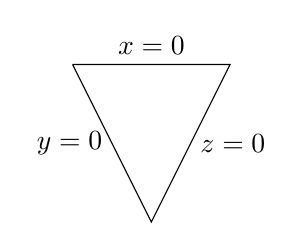
\begin{tikzpicture}[
    tlabel/.style={pos=0.4,right=-1pt},
    baseline=(current bounding box.center)
    ]
\draw (0,0) -- (2,0) node[midway, above] {$x=0$}
   -- (1,-2) node[midway,right] {$z=0$}
   -- (0,0) node[midway,left] {$y=0$}; 
\end{tikzpicture}
$\begin{tikzcd}
 \arrow[rrr, bend left] &  &  &  \arrow[lll, bend left]
\end{tikzcd}$
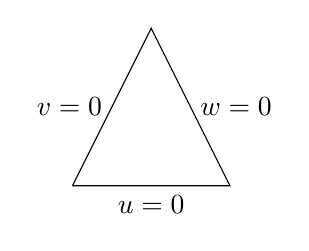
\begin{tikzpicture}[
    tlabel/.style={pos=0.4,right=-1pt},
    baseline=(current bounding box.center)
    ]
\draw (0,0) -- (2,0) node[midway, below] {$u=0$}
   -- (1,2) node[midway,right] {$w=0$}
   -- (0,0) node[midway,left] {$v=0$}; 
\end{tikzpicture}
\end{center}
\begin{center}
\begin{tikzcd}
 \arrow[rd, bend left] &                        \\
                       &  \arrow[lu, bend left]
\end{tikzcd}
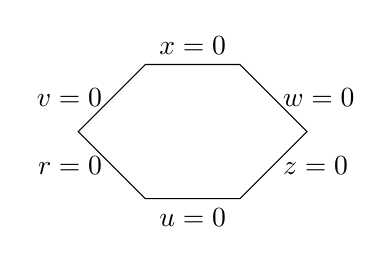
\begin{tikzpicture}[
    tlabel/.style={pos=0.4,right=-1pt},
    baseline=(current bounding box.north)
    ]
\draw (0,0) -- (1.2,0) node[midway, below] {$u=0$}
   -- (2.052,.852) node[midway,right] {$z=0$}
   -- (1.2,1.704) node[midway,right] {$w=0$}
   -- (0,1.704) node[midway,above] {$x=0$}
   -- (-.852,.852) node[midway,left] {$v=0$}
   -- (0,0) node[midway,left] {$r=0$}; 
\end{tikzpicture}
$\bigne$
\end{center}
This  hexagon is called the \textit{del Pazzo surface of degree three}, denoted by $\mathrm{dP}_3$. Each of its lines is isomorphic to $\P^1$. 
\end{exmp}


\begin{note}
Suppose that $C$ is a smooth curve and that $\dim{X} < 2$. Then $\varphi : C \setminus \pt \to X$ automatically extends.  But if $C$ were singular or $\dim{X} \geq 2$, then this would be false.
\end{note}

\subsection{Lecture 9}

\begin{defn}[Picard group]
Let $X$ be a complex manifold. The \textit{Picard group $\pic(X)$ of $X$} is the group of all isomorphism classes of line bundles over $X$ under $\otimes$.
\end{defn}

Let $n\in \N$ and consider the family of line bundles $\left\{\O(k) \mid k \in \Z\right\}$ over $\P^n$.

\begin{prop}
$\pic\left(\P^n\right) \cong \Z$ with generator $\O(1)$. 
\end{prop}

Let $\P^n = \P(V)$. We have an exact sequence
\[
\begin{tikzcd}
0 \arrow[r] & L \arrow[r] & \O_{\P^n}\otimes_{\C} V \arrow[r] & \cdots
\end{tikzcd}
\]
We have that
\be
\item $\Gamma\left(\P^n , \O(1)\right) = \C\langle z_0, \ldots, z_n\rangle = V^{\vee}$,
\item $\Gamma \left(\P^n, \O({-1})\right) =0$, and
\item $\Gamma \left(\P^n, \O(k)\right) = \begin{cases} \sym^k\left(V^{\vee}\right) & k\geq0 \\ 0 & k<0\end{cases}$.
\ee

Let $U_i = \left\{z \in \P^n \mid z_i \ne 0\right\}$ for each $i\in \left\{0, 1, \ldots, n\right\}$, so that $\P^n = \bigcup_{i=0}^n$. Let $Z_{ij} = \frac{z_j}{z_i}$, thereby endowing each $U_i$ with local coordinates. Let $s$ be a section of $\O$, so that $$s = \left(s_i \in \Gamma\left(U_i, \O\right)\right)_{i=0}^n.$$ Note that $Z_i$ defines a section on $U_j$ with $s_j = \frac{z_i}{z_j} = Z_{ji}$ for each $j=0, \ldots, n$. 
\[
\begin{tikzcd}
s_j \arrow[r, equals] \arrow[d, equals]   & Z_{jk}\cdot s_k \arrow[d, equals]  \\
\frac{z_i}{z_j} \arrow[r, equals] & Z_{jk}\cdot\frac{z_i}{z_k}
\end{tikzcd}
\]
We can establish the following properties.
\be
\item If $\O= \O(1)$, then $s_i = Z_{ij}s_j$.
\item If $\O = \O({-1})$, then $s_i = Z_{ji}s_j$.
\item If $\O = \O(k)$, then $s_i = \left(Z_{ij}\right)^ks_j$.
\ee

In summary,

\begin{table}[H]
\centering
\begin{tabular}{c|c|c|c|c}
 & $\O$ (trivial) & $\O({-1})$ & $\O(1)$ & $\O(k)$ \\ \hline
LB & $\P^n \times \C$ & tautological & dual &  \\ \hline
Sheaf & $1$ & $Z_{ji}$ & $Z_{ij}$ & $\left(Z_{ij}\right)^k$ \\ \hline
Divisor & $0$ & ${-}\underset{\text{h.p.}}{H}$ & $+H$ & $k{H}$ \\ \hline
Map & $\pt$ & undefined & $\id$ & \begin{tabular}[c]{@{}c@{}}$\begin{cases} \text{Veronese} & k>0\\ \\ \text{undefined} & k <0\\ \\ \pt & k=0\\ \end{cases}$\end{tabular}
\end{tabular}
\end{table}

Let $X$ be a complex $n$-manifold. Then $T_X$ consists of all local sections on an open set $U$ with coordinates, say, $z_1, \ldots, z_n$. The set $\left\{\frac{\partial}{\partial{z_i}}\right\}$ is a basis for this, with each section of the form $\sum_{i=1}^n f_i\frac{\partial}{\partial{z_i}}$ where each $f_i$ belongs to $\Gamma\left(U, \O\right)$. For any other basis $\left\{\frac{\partial}{\partial{w_i}}\right\}$, we have that 
\[
\frac{\partial}{\partial{w_i}} = \sum\frac{\partial{z_j}}{\partial{w_i}}\frac{\partial}{\partial{z_j}}.
\] Note that  $T_V \cong \O_V \otimes_{\C} V$. In general,  $\Omega_V^i \cong \O_V \otimes \bigwedge^i V^{\vee}$.
\begin{question}
What is $T_{\P(V)}$?
\end{question}


\begin{note}[Bundle associated to an $n$-manifold] $ $
\be
\item $T_X^{\vee} = \Omega \equiv \Omega^1$, whose transition functions are precisely the inverses of the transposes of those for $T_X$. 
\item Let $\Omega^i = \bigwedge^i{\Omega^1}$.  If $i=n$, then we call this space the \textit{canonical sheaf $K_X$} or the \textit{dualized sheaf $\omega_X$}.
\item Recall the map $\bigwedge^i : \GL(n) \to \GL{n\choose i}$. If $i=n$, then this is precisely the determinant map.
\ee
\end{note}

Consider the exact sequence
\[
\begin{tikzcd}
0 \arrow[r] & \O \arrow[r]         & \O(1)^{\oplus{n+1}} \arrow[r]       & T_{\P^n} \arrow[r]                     & 0 \\
            & 1 \arrow[r, maps to] & \left(z_i\right)                    &                                        &   \\
            &                      & \left(a_i\right) \arrow[r, maps to] & \sum a_i\frac{\partial}{\partial{z_i}} &  
\end{tikzcd}
.\]

\begin{term}
The vector field given by $\sum z_i\frac{\partial}{\partial{z_i}}$ is known as the \textit{Euler vector field}.
\end{term}

Moreover, we have a commutative diagram
\[
\begin{tikzcd}
0 \arrow[r] & \underbrace{\O_{\P(V)}}_{\C} \arrow[r] & \underbrace{\O_{\P(V)}(1)}_{V^{\vee}}\otimes V \arrow[r] \arrow[d, hook] & T_{\P(V)} \arrow[r] \arrow[d, hook] & {,} \\
            &                                        & \O_V(1)\otimes V \arrow[r, "\cong"]                                      & T_V \arrow[r]                       & 0  
\end{tikzcd}
.\]
\begin{term} 
The top row of this diagram is known as the \textit{Euler sequence}.
\end{term}
Therefore, the \textit{weight} of $V$ equals ${-1}$, whereas the weight of $V^{\vee}$ equals ${+}1$.

\medskip

Informally, any holomorphic function $f$ on $V$ is the same as a direct sum of homogenous functions of degree $k$, i.e., has the form
\[
\bigoplus_{k-0}^{\infty} \Gamma\left(\P(V), \O(k)\right),
\]
called the \textit{Taylor expansion of $f$}.

\begin{note}
In general, we have an exact sequence
\[
\begin{tikzcd}
0 \arrow[r] & \O(n) \arrow[r] & \O^{\left(n+1\right)} \arrow[r] & T_{\P}\left({-1}\right) \arrow[r] & 0
\end{tikzcd}
,\] which becomes the Euler sequence
\[
\begin{tikzcd}
0 \arrow[r] & \O \arrow[r] & \O(1)\oplus \O(1) \arrow[r] & T_{\P^1} \arrow[r] & 0
\end{tikzcd}
\] in the case where $n=1$. It follows that 
\[
K_{\P^n} = \O_{\P^n}\left({-n}-1\right).
\]
\end{note}

\begin{lemma}
If $0 \to A \to B \to C \to 0$ is an exact sequence of vector spaces, then $$\det(B) = \det(A) \otimes \det(C).$$
\end{lemma}

\begin{corollary}
$\O(2) \cong \det \left(\O(1) \oplus \O(1)\right) =\det(\O) \otimes \det(T) = \det(T)$.
\end{corollary}

\begin{remark}
Similarly, we can show that $\det\left(T_{\P^n}\right) =\O_{\P^n}(n+1)$.
\end{remark}

\medskip

Suppose that $X\subset Y$ is a submanifold of codimension $1$. Then we have a short exact sequence
\[
\begin{tikzcd}
0 \arrow[r] & T_X \arrow[r] & \left(T_Y\right)\bigr\rvert_X \arrow[r] & N_{X\mathbin{/}Y} \arrow[r] & 0
\end{tikzcd}.
\]

\begin{lemma}\label{norm}
$N_{X\mathbin{/}Y} \cong \O_Y\left(X\right)\bigr\rvert_X$.
\end{lemma}

In other words, if $L\in \pic(Y)$, $s\in \Gamma\left(Y, L\right)$, and $X = \left\{s=0\right\}$, then $N_{X\mathbin{/}Y} \cong L\bigr\rvert_X$.

\begin{theorem}[Adjunction formula]
$K_X \cong \left(K_Y \otimes_{\O_Y} \O_Y(X)\right)\bigr\rvert_X$.
\end{theorem}
\begin{proof}
Note that $\left(K_Y^{-1}\right)\bigr\rvert_X = K_X^{-1} \otimes N_{X\mathbin{/}Y}$. Thus,
\begin{align*}
K_X & \cong K_Y\bigr\rvert_X \otimes N_{X\mathbin{/}Y}  
\\ & \cong K_Y\bigr\rvert_X \otimes  \O_Y(X)\bigr\rvert_X
\\ & \cong \left(K_Y \otimes \O_Y(X)\right)\bigr\rvert_X
.\end{align*}
\end{proof}


\subsection{Lecture 10}

\begin{proof}[Proof of \cref{norm}]
Let $s\in \Gamma\left(Y, L\right)$. We can write $s = f{s_0}$, so that $d{s} = s_0d{f} + fd{s_0}$. Consider the short exact sequence
\[
\begin{tikzcd}
0 \arrow[r] & T_X \arrow[r] & T_Y\bigr\rvert_X \arrow[r, "ds"] & L \arrow[r] & 0
\end{tikzcd}.
\] Thus, $ds$ transforms just as $s_0$ does.
\end{proof}


\begin{exmp} $ $
\be
\item Let $Y = \P^3$. Suppose that $\widetilde{X}$ is a smooth curve of degree $d$. Then $K_Y = \O\left({-3}\right)$, and  $K_X = \O\left(d-3\right)\bigr\rvert_X$. Further, if $g$ denotes the genus of a surface, then B\'ezout's theorem implies that
\begin{align*}
2g-2  = \deg & \left( K_X\right) =d\left(d-3\right)
\\ &  \Downarrow
\\ g  = 1+ \frac{d\left(d-3\right)}{2}&= \frac{\left(d-1\right)\left(d-2\right)}{2}.
\end{align*}
In particular,
\begin{table}[H]
\centering
\begin{tabular}{l|l}
$d$ & $g$ \\ \hline
1 & 0 \\
2 & 0 \\
3 & 1 \\
4 & 3 \\
5 & 6
\end{tabular}
.\end{table}
\item Let $Y = \P^n$ and let $X\subset Y$ be of dimension $d$. Note that $K_X = \O_X$ precisely when $d= n+1$. In particular,
\begin{table}[H]
\centering
\begin{tabular}{l|l}
$n$ & $X$ \\ \hline
2 & cubic / elliptic curve \\
3 & quartic (\textit{a $K_3$ surface}) \\
4 & quintic
\end{tabular}
.\end{table}
\ee
\end{exmp}

\smallskip

Let $p_1, \ldots, p_n \in \P^N$,  let $m_1, \ldots, m_n \in \Z_{\geq 1}$, and let $d\in \Z$. We wish to describe $$\Gamma \left(\J_{\Sigma_{m_ip_i}}\left(d\right)\right) \coloneqq \left(\J_{\Sigma_{m_ip_i}} \otimes \O(d) \right).$$ For simplicity, let $N=2$.

\begin{defn}
If $n=1$, then \textit{imposition} is $\imp_m \equiv \codim\left(\Gamma\left(\J_{mp}(d), \Gamma\left(\O(d)\right)\right)\right)$.
\end{defn}

\begin{prop}
$\imp_m = {{m+1} \choose 2}$. 
\end{prop}

\begin{defn} Consider the space $\Gamma$.
\be
\item The \textit{actual dimension of $\Gamma$} is the dimension of $\Gamma$ as a vector space.
\item The \textit{virtual dimension $\vd\left(\Gamma\right)$ of $\Gamma$} is the quantity ${{d+2}\choose 2}-1 - \sum_i{{m_i+1}\choose 2}$.
\item The \textit{expected dimension of $\Gamma$} is the quantity $\max\left(\vd\left(\Gamma\right), 0\right)$.
\ee
\end{defn}

\begin{conj}\label{c1}
The actual dimension always equals the expected dimension.
\end{conj}
\begin{proof}[Answer]
This is \textbf{false}. For example, let $N=2$, $d = 1$, $m_i =1$, and $n=3$. Then $\Gamma =0$, so that $\P\left(\Gamma\right) =\emptyset$. Hence the expected dimension is zero, but the actual dimension is positive whenever the $p_i$ are co-linear.
\end{proof}

This leads us to the following modification of \cref{c1}.

\begin{conj}\label{c2}
If the $p_i$ are in \textit{general position}, then the actual dimension equals the expected dimension.
\end{conj}
\begin{proof}[Answer]
This is \textbf{false}. To see this, let $d=2$ and $N= n = m_i=2$. Consider a conic $C$ through five points. Here, our conjecture holds. But if instead $N=2$, $d=4$, $n=5$, and $m_i=2$, then the virtual dimension is precisely ${{4+2}\choose 2}-5\cdot 3 =0$. Since the square of $C$ exists, it follows that our conjecture fails.
\end{proof}

We can improve \cref{c2} as follows.

\begin{conj}
If the actual dimension is different from the expected dimension, then $\Gamma\left(\J_{\sum_{m_ip_i}}(d)\right)$ has a base curve.
\end{conj}
\begin{proof}[Answer]
This is \textbf{unknown}. See the article \href{https://pdfs.semanticscholar.org/3db0/6dd64b62f15f04c9caa13dba2db7ca4d9fdd.pdf}{``Linear Systems of Plane Curves"} by Rick Miranda.
\end{proof}

Consider the map $\left\lvert{\O(d)}\right\rvert : \P^2 \hookrightarrow \P^{{{d+2}\choose 2} -1}$. We also have a map
\[
\begin{tikzcd}[column sep = large]
                                                    & \P^2 \arrow[r, "\left\lvert{\J_{\sum_{p_i}(d)}}\right\rvert", dashed] & \P^{\dim -1} \\
{\bl_{p_1, \ldots, p_n}\left(\P^2\right)} \arrow[r, equals] & \widetilde{\P^2} \arrow[u] \arrow[ru]                      &             
\end{tikzcd}
\]

\begin{prop}
Consider the blow-up $\pi : \underbrace{\widetilde{\P^2}}_{X} \to \P^2$. We have that $$\pic(X) \cong \Z\langle \pi^{\ast}\left(\O(1)\right), E_1, \ldots, E_n\rangle$$ where $E_i$ denotes the divisor collapsing to $p_i$.
\end{prop}

\begin{remark} $ $
\be
\item[Good:] $\pi^{\ast}{\O(d)} - \sum{m_iE_i} \longleftrightarrow \J_{\sum{m_ip_i}}(d)$.
\item[Better:] $\Gamma\left(X, \text{\textquotesingle\textquotesingle}\right) = \Gamma\left(\P^2, \text{\textquotesingle\textquotesingle}\right) $.
\item[Best:] $\pi_{\ast}\left( \text{\textquotesingle\textquotesingle}\right) =  \text{\textquotesingle\textquotesingle}$.
\ee
\end{remark}

\begin{conj}
Any line bundle $L \coloneqq \left(\pi^{\ast}{\O(d)} -\sum{m_iE_i}\right)$ has the expected dimension of the space of sections unless $\BL\left(L\right)$ contains a $\left({-1}\right)$-curve, i.e., a smooth curve $C$ of genus zero  such that $C^2 = {-1}$.
\end{conj}

\begin{exmp}[$\left({-1}\right)$-curve]
Let $d=1$, $n=2$, and $m_1=m_2 =1$. If $C\in \O(1)({-p}-q)$, then $C^2 =1^2 -1-1 = {-1}$. In general, 
\[
\O(d)\left (\left({-\sum m_IE_i}\right)\left(\O(d) -\sum m_ip_i\right)\right) = dd' -\sum{m_im_i'}.
\] In $\P^2$, this means the number of intersections other than the $p_i$.
\begin{table}[H]
\centering
\begin{tabular}{c|c}
Space & $C^2$ \\ \hline
$\O(1)$ & $1$ \\
$\O(1)({-p})$ & $0$ \\
$\O(1)({-p}-q)$ & ${-1}$ \\
\vdots &  \\
$\O(2)$ & $4$ \\
$\O(2)\left({-p}_1\right)$ & $3$ \\
$\O(2)\left({-p_1} -p_2\right)$ & $2$ \\
\vdots &  \\
$\O(2)\left({-p_1} -\cdots - p_4\right)$ & $0$ \\
$\O(2)\left({-\sum_{i=1}^5 p_i}\right)$ & ${-1}$
\end{tabular}
\end{table}
\end{exmp}

\section{K\"ahler manifolds}

\subsection{Lecture 11}

Consider the following Hasse diagram of subgroups:

\begin{center}
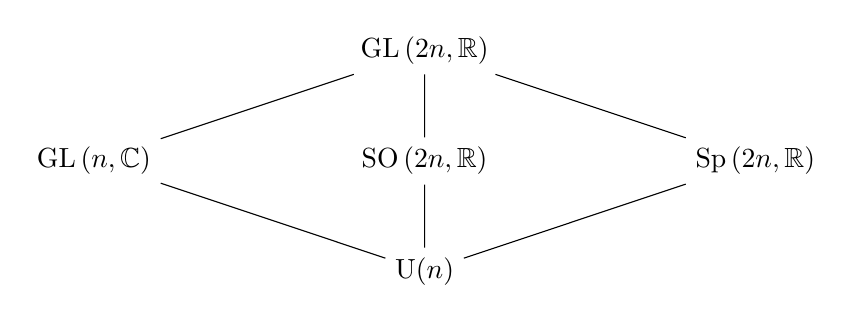
\begin{tikzpicture}[scale=.7]
  \node (one) at (0,2) {$\GL\left(2n, \R\right)$};
  \node (a) at (-6,0) {$\GL\left(n, \C\right)$};
  \node (b) at (0,0) {$\SO\left(2n, \R\right)$};
  \node (d) at (6,0) {$\Sp\left(2n, \R\right)$};
  \node (zero) at (0,-2) {$\U(n)$};
  \draw (zero) -- (a) -- (one) -- (b) -- (zero) -- (d) -- (one);
\end{tikzpicture}
\end{center}

where $\Sp\left(2n, \R\right)$ denotes the group of real $2n\times 2n$ \textit{symplectic matrices}, i.e., matrices $M$ satisfying $$M^t{\begin{bmatrix} 0 & I_n \\ {-I_n} & 0 \end{bmatrix}}{M} = \begin{bmatrix} 0 & I_n \\ {-I_n} & 0 \end{bmatrix}.$$

Similarly, we can view various areas of geometry as refinements of certain others. Specifically,

\begin{center}
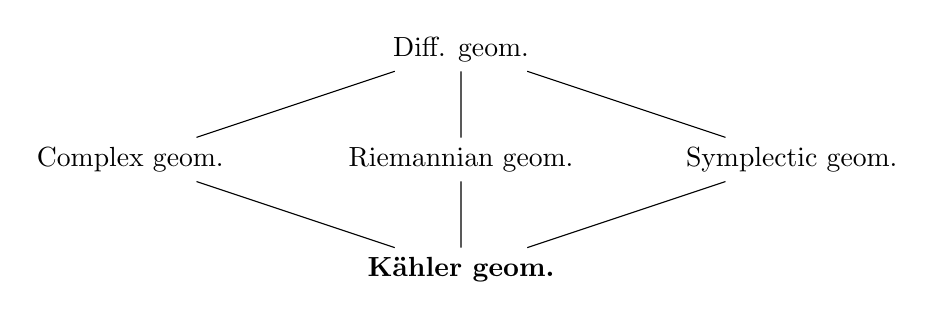
\begin{tikzpicture}[scale=.7]
  \node (one) at (0,2) {Diff. geom.};
  \node (a) at (-6,0) {Complex geom.};
  \node (b) at (0,0) {Riemannian geom.};
  \node (d) at (6,0) {Symplectic geom.};
  \node (zero) at (0,-2) {\textbf{K\"ahler geom.}};
  \draw (zero) -- (a) -- (one) -- (b) -- (zero) -- (d) -- (one);
\end{tikzpicture}
\end{center}

Before investigating K\"ahler geometry, we establish some basic geometric concepts.

\begin{defn}
Let  $X$ be a real manifold. An \textit{almost complex structure on $X$} is a bundle map $I : T{X} \to T{X}$ such that $I^2 = {-1}$.
\end{defn}

Note that the eigenvalues of $I$ are precisely $i$ and ${-i}$.

\begin{notation} $ $
\be
\item Let $T^{1,0}$ denote the eigenspace of $i$.
\item  Let $T^{0,1}$ denote the eigenspace of ${-i}$.
\ee
\end{notation}

Any complex manifold $X$ has a natural almost complex structure. Indeed, given local coordinates $x_i, y_i$ on $X$, define $I$ by $\frac{\partial}{\partial{x_i}} \mapsto \frac{\partial}{\partial{y_i}}$ and $\frac{\partial}{\partial{y_i}} \mapsto {-\frac{\partial}{\partial{x_i}}}$. It follows that any manifold with an almost complex structure has even dimension.

\medskip

Now, consider the  complexification of our tangent bundle, $T^{\C}{X} \equiv T{X} \otimes_{\R}\C$.  

\begin{prop} $ $
\be
\item $T^{\C}{X} \cong T^{1,0} \oplus T^{0,1}$.
\item $T^{\ast{\C}}{X} \cong T^{\ast{1,0}}\oplus T^{\ast{0,1}}$
\ee
\end{prop}

Define, formally, the complex coordinates $z_j = x_j + iy_j$. Note that $T^{\C}{X}$ has as basis $\left\{\frac{\partial}{\partial{z_j}}, \frac{\partial}{\partial{\bar{z}_j}}\right\}$ and that $T^{\ast{\C}}{X}$ has as basis $\left\{d{z_j}, d{\bar{z}_j}\right\}$ where $d{z_j} \equiv d{x_j} + id{y_j}$.

\begin{notation} $ $
\be
\item $\bigwedge^k{X} \coloneqq \bigwedge^k{T^{\ast}{X}}$.
\item $\bigwedge^{p,q}{X} \coloneqq \bigwedge^p{T^{\ast{1,0}}}{X} \otimes_{\C} \bigwedge^q{T^{\ast{0,1}}}{X}$.
\ee
\end{notation}

\begin{note}\label{decomp} Let $X$ be an $n$-dimensional complex manifold.
\be
\item $\left(\bigwedge^k{T^{\ast}{X}}\right) \otimes \C = \bigwedge^k_{\C}\left(T^{\ast}{X} \otimes \C\right)$.
\item $\left(\bigwedge^k{X}\right) \otimes \C = \bigoplus_{p+q = k} \bigwedge^{p,q}{X}$.
\ee
\end{note}

Therefore,  $\left(\bigwedge^k{X}\right) \otimes \C$ can be decomposed according to the counting equation ${2n \choose k} = \sum{{n\choose p}{n\choose q}}$.

\medskip

Let $U$ and $V$ be open  in $\C^n$. Let $f: U \to V$ be holomorphic. Then the map $d{f} : T{U} \to T{V}$ extends to a map $d{f}^{\C} : \T^{\C}{U} \to T^{\C}{V}$ that preserves both $T^{1,0}$ and $T^{0,1}$. 

\medskip

Let $\A^{p,q}  = \Gamma\left(\bigwedge^{p,q}\right)$, i.e., $\A^{p,q}\left(U\right) = \Gamma\left(U, \bigwedge^{p,q}\right)$. Consider the exterior derivative $d: \A^k \to \A^{k+1}$. With $\pi$ denoting the projection map, define the operators
\begin{align*}
\partial & = \pi^{p+1, q} \circ d
\\ \bar{\partial}  & = \pi^{p, q+1} \circ d
\end{align*}

on $A^{p,q}$. Locally, we have that $$df = \frac{\partial{f}}{\partial{x_i}}d{x_i} + \frac{\partial{f}}{\partial{y_i}}d{y_i} = \frac{\partial{f}}{\partial{z_i}}d{z_i} + \frac{\partial{f}}{\partial{\bar{z}_i}}d{\bar{z}_i} $$ for any $f\in \A^{0,0}$.  By the Cauchy-Riemann equations, it follows that $f$ is holomorphic if and only if $\bar{\partial}{f} = 0$.

\begin{remark}
Any $\left(p,q\right)$-form locally looks like $f_{IJ}d{z_I}\wedge \bar{z}_J$.
\end{remark}

\begin{prop} $ $
\be
\item $d = \partial + \bar{\partial}$.
\item $\partial^2 =0 = \bar{\partial}^2$. 
\item $\partial{\bar{\partial}} = {-\bar{\partial}{\partial}}$.
\item $\partial\left(\alpha \wedge \beta\right) = \partial{\alpha} \wedge \beta + \left({-1}\right)^{p+q} \alpha \wedge \partial{\beta}$ for any $\alpha \in \A^{p,q}$ and $\beta \in \A^{r,s}$.
\ee
\end{prop}

\begin{lemma}[Single-variable Poincar\'e]
Consider the disk $B_{\epsilon} \subset \overline{B_{\epsilon}} \subset U \subset \C$ where $U$ is open.  Let $\alpha = f{d{\bar{z}}} \in \A^{0,1}\left(U\right)$ and $$ g(z) = \frac{1}{2\pi i}\int_{\overline{B_{\epsilon}}}\frac{f(w)}{w-z}{d{w} \wedge d{\bar{w}}}.$$ Then $\bar{\partial}{g} = \alpha$. 
\end{lemma}

\begin{lemma}[Multi-variable Poincar\'e]
Consider the polydisk $B_{\epsilon} \subset \overline{B_{\epsilon}} \subset U \subset \C^n$  where $U$ is open. Let $\alpha \in \A^{p,q}$ with $q>0$ and $\bar{\partial}{\alpha} =0$. Then there is some $\beta \in \A^{p, q-1}\left(B_{\epsilon}\right)$ such that $\bar{\partial}{\beta} = \alpha$.
\end{lemma}

\begin{remark}
If $U$ is contractible, then any differential form on $U$ is closed if and only if it is exact.
\end{remark}

Let $U \subset \C^n$ be open and let $I$ denote the natural almost complex structure on $U$. Let $g$ be a Riemannian metric on $U$.

\begin{defn}[Hermitian metric] $ $
\be
\item  We say that $g$ is \textit{compatible with $I$} or \textit{(almost) Hermitian} if $g\left(u,v\right) = g\left(I{u}, I{v}\right)$.
\item If $g$ is Hermitian, then the real $\left(1,1\right)$-form $\omega \in \A^{1,1}\left(U\right) \cap \A^2\left(U\right)$ defined by $$\omega\left(u,v\right) = g \left(I{u}, v\right)$$ is called the \textit{fundamental form of $g$}.
\ee
\end{defn}

\begin{notation}
$h \coloneqq g -i{\omega}$.
\end{notation}

\begin{defn}
A Hermitian matrix $M$ is \textit{positive-definite} if $z^{\ast}Mz >0$ for every nonzero complex column vector $z$.
\end{defn}

Note that $h$ is a positive-definite form in the sense that, locally, its component functions define a positive-definite matrix at any given point. 

\begin{exmp}
Let $g = \underbrace{d{x^2}}_{d{x}\otimes d{x}} + d{y^2} = \sum_{i=1}^nd{x_i^2} + d{y_i^2} \in T^{\ast}\otimes T^{\ast} \subset \left(T^{\ast}\otimes T^{\ast}\right)\otimes_{\R}\C$. Since
\[
d{z} \wedge d{\bar{z}} = \left(d{x} + id{y}\right) \wedge \left(d{x}- id{y}\right) = {-2id{x}}\wedge d{y}
,\]
it follows that
\[
\omega = d{x}\otimes d{y} -d{y}\otimes d{x} = \frac{i}{2}d{z} \wedge d{\bar{z}}
.\] Moreover, we see that
\begin{align*}
h & = z-i{\omega}
\\ & = d{x^2} -id{x}d{y} +id{y}d{x} +d{y}^2
\\ & = d{x}\left(d{x}-id{y}\right) + id{y}\left(d_x+-id{y}\right)
\\ & = \left(d{x} + id{y}\right)\left(d{x}-id{y}\right) 
\\ & = d{z}\otimes d{\bar{z}}.
\end{align*}
\end{exmp}

For each $z\in \C^n$, define the matrix $\left(h_{ij}\right)\left(z\right)$ by $$h_{ij}\left(z_1, \ldots, z_n\right) = h\left(\frac{\partial}{\partial{x_i}}, \frac{\partial}{\partial{x_j}}\right).$$ 

\begin{prop}
Let $I$ be an almost complex structure on $U\subset X$ and let $g$ be compatible with $I$. Then $d{\omega} =0$ if and only if for each $x\in X$, there exist a neighborhood  $U'$ of $x$ and a holomorphic map $f: U' \to U$ such that $f^{\ast}{g}$ \textit{oscillates the standard metric to the second order}, i.e., $\left(h_{ij}\right) = \id + O\left(\left\lvert{z}\right\rvert^2\right)$.
\end{prop}

\begin{notation}
In this case, we write $h \approx \id$.
\end{notation}

\begin{defn}[K\"ahler manifold]
Consider the four-tuple $\left(X, I, g, \omega\right)$.  We say that $X$ is a \textit{K\"ahler manifold} if $d{\omega}=0$. In this case, we call $g$ a \textit{K\"ahler metric on $X$} and $\omega$ a \textit{K\"ahler form}.
\end{defn}

\begin{defn}
Let $\left(X, I, g, \omega\right)$ be a K\"ahler structure with $\dim{X} =n$.
\be
\item The \textit{Lefschetz operator} $L: \bigwedge^k{X} \to \bigwedge^{k+2}{X}$ is defined by $\alpha \mapsto \alpha \wedge \omega$.
\item The \textit{Hodge $\ast$-operator} $\ast : \bigwedge^k{X} \to \bigwedge^{2n-k}{X}$  is defined by the property
\[
\alpha \wedge \ast{\beta} = \hat{g}\left(\alpha, \beta\right){\omega^n}
\] where $\hat{g}$ is induced by $g$ and $\omega^n$ denotes the (positively oriented) volume form on $X$.
\item  The \textit{dual Lefschetz operator} $\Lambda : \bigwedge^k{X} \to \bigwedge^{k-2}{X}$ is defined as the composite $\ast^{-1} \circ L\circ \ast$.
\ee
\end{defn}

\begin{note} $ $
\be
\item In coordinates for which $h\approx \id$, we have that $\ast{d{x^I}} = d{x^{\partial}}$ where $\partial \coloneqq I^{\C}$ ??.
\item $\Lambda$ is $\O$-linear.
\ee
\end{note}

\subsection{Lecture 12}

\begin{prop}
Let $X$ be a complex manifold. Let $\omega$ be a closed real positive-definite form of type $\left(1,1\right)$, i.e., locally, $\omega = \frac{i}{2}\sum h_{ij}d_{z_i}\wedge d{\bar{z}_j}$ such that the matrix $\left(h_{ij}(p)\right)$ is positive-definite for each $p$. Then there exists a K\"ahler metric $g$ on $X$ such that $\omega$ equals the fundamental form of $g$. 
\end{prop}

Since every K\"ahler form is positive-definite, it follows that the set $\K_X$ of all K\"ahler forms on $X$ is precisely the set of all closed real positive-definite forms of type $\left(1,1\right)$.

\begin{defn}
Let $V$ be a vector space over $\R$. A subset $C\subset V$ is a \textit{convex cone} if $av_1 + bv_2 \in C$ for any $v_1, v_2\in C$ and any $a,b\in \R_{>0}$.
\end{defn}

\begin{corollary}
Suppose that $X$ is compact. Then $\K_X$ is an open convex cone in the infinite-dimensional real vector space $S\coloneqq \left\{\omega \in \A^{(1,1)}\left(X\right) \cap \A^2\left(X\right) \mid d{\omega} =0\right\}$.
\end{corollary}
\begin{proof}[Idea]
The fact that $\K_X$ is a convex cone follows from the fact that the set of all positive-definite matrices is a convex cone. It remains to show that $\K_X$ is open. Since $X$ is compact, it has a finite open cover $\left\{U_i\right\}$. The set $P_{U_i}\subset S$ of all  forms that are positive-definite on $U_i$ is open. Thus, $\bigcap_i P_{U_i} = \K_X$  is also open.
\end{proof}

\begin{remark}
It turns out that $S \cong H^2\left(X, \R\right)$.
\end{remark}

\begin{exmp}\label{km1} $ $
\be
\item The form $\omega \equiv \frac{i}{2}d{z} \wedge d{\bar{z}}$ is K\"ahler on $\C$ and is exact.
\item The same form descends to a K\"ahler form on the torus $\C/\Lambda$, which is not exact. 
\item Consider the inclusion $i : X \to Y$ of a closed submanifold. If $\omega$ is K\"ahler on $Y$, then $i^{\ast}{\omega}$ is K\"ahler on $X$.
\ee
\end{exmp}

\begin{note}
Let $f: X \to Y$ be holomorphic and let $\omega$ be a K\"ahler form on $Y$. It is \emph{not} necessarily true that $f^{\ast}{\omega}$ is K\"ahler on $X$. For example, if $f(x) = \pt$ for all $x\in X$, then $f^{\ast}{\omega}$ is the zero form and thus not positive. 
In general,  $f$ must be injective. For example, if $f: C \to \C$ is a double cover where $C$ is a Riemann surface, then $C$ inherits a K\"ahler form only outside the  \textit{ramification of $f$}, i.e., the set $$\left\{c\in C \mid \text{there is no neighborhood } U \text{ of  } c \text{ such that } f\restriction_U \text{ is injective}\right\}.$$ This is precisely the set of points at which $d{f}$ is nonzero.
\end{note}

\begin{exmp}\label{km2} $ $
\be
\item  Consider the open cover $\left\{U_i\right\}_{1\leq i \leq n}$ of $\P^n$ where $U_i \equiv \left\{z \in \P^n \mid z_i \ne 0\right\}$. Define $\varphi_i : U_i \overset{\cong}{\longrightarrow} \C^n$ by $$\left(z_0, \ldots, z_n\right) \mapsto \underbrace{\left(\frac{z_0}{z_i}, \ldots, \frac{z_{i-1}}{z_i}, \frac{z_{i+1}}{z_i}, \ldots, \frac{z_n}{z_i}\right)}_{\left(w_1, \ldots, w_n\right)}. $$ Then $\left\{\left(U_i, \varphi_i\right)\right\}$ is a holomorphic atlas on $\P^n$. For each $i$, let 
\[
\omega_i =  \frac{i}{2\pi}{\partial{\bar{\partial}}\log\left(\sum_{l=0}^n \left\lvert{\frac{z_l}{z_i}}\right\rvert^2\right)}
.\] By way of $\varphi_i$, this becomes
\[
\frac{i}{2\pi}{\partial{\bar{\partial}}\log\left(1+ \sum_{k=1}^n \left\lvert{w_k}\right\rvert^2\right)}
.\]
\begin{exercise}
 Show that $\omega_i\restriction_{U_i \cap U_j} = \omega_j\restriction_{U_i \cap U_j}$.
\end{exercise}
Therefore, the $\omega_i$ patch together to form a metric $\omega$ on $\P^n$, known as the \textit{Fubini-Study metric}. 
\begin{exercise}
Show that $\omega$ is closed, real, positive, and of type $\left(1,1\right)$.
\end{exercise}
It follows that $\omega$ is a K\"ahler metric.

\item  Any branched cover of $\P^n$ admits a K\"ahler metric (which must be different from the pullback of a K\"ahler metric on $\P^n$). For example, consider an elliptic curve $E \to \P^1$, which fits into a commutative sqaure
\[
\begin{tikzcd}
E \arrow[d, equals] \arrow[r] & \P^1                   \\
E \arrow[r, hook]     & \P^2 \arrow[u, dashed]
\end{tikzcd}
.\]
\ee
\end{exmp}

\begin{defn}
A complex manifold is \textit{projective} if it is isomorphic to a closed submanifold of projective space.
\end{defn}

\begin{prop}
Any projective complex manifold is K\"ahler.
\end{prop}
\begin{proof}
This follows from \cref{km1}(3) together with \cref{km2}(1).
\end{proof}


\begin{defn} $ $
Let $X$ be  a complex manifold. Let $D$ be a first-order operator on $\A^{\ast}\left(X\right)$.  
\be 
\item The \textit{adjoint of $D$} is
\[ 
D^{\ast} \equiv {-\ast} \circ D \circ \ast 
\]
\item The \textit{Laplacian associated to $D$} is 
\[
\Delta_D \equiv D{D^{\ast}} + D^{\ast}{D}.
\]
\ee
\end{defn}

\begin{defn}
The \textit{Laplace operator} is $\Delta \equiv d{d^{\ast}} + d^{\ast}{d}$.
\end{defn}

\begin{exmp} $ $
\be
\item Let $D = \partial$. Then $\partial^{\ast}\left(f_{IJ}d{z}^I \wedge d{z}^J\right) = \sum_{i\in I}f_{IJ}d{z}^{I-i}\wedge d{\bar{z}}^J$.
\item Let $D = d$. Let $\left(x_1, \ldots, x_n\right)$ be local coordinates on $X$. Then
\begin{align*}
d\left(fdx^I\right) & = \sum_{i\notin I} \frac{\partial{f}}{\partial{x_i}}d{x^n}\wedge d{x}^I
\\  d^{\ast}\left(fdx^I\right) & =  \sum_{i\in I}\frac{\partial{f}}{\partial{x_i}}d{x}^{I-i}.
\end{align*}
Therefore,
\begin{align*}
d\circ d^{\ast}\left(fdx^I\right)  & = \frac{\partial^2}{\partial{x_i}\partial{x_j}}d{x}^{I-i \cup j}
\\ & = \sum_{\substack{i\in I \\ j \notin I}}\cdots +\sum_{i=j \in I}\cdots.
\\ d^{\ast}\circ d\left(fd{x}^I\right) &=0 + \sum_{i=j\notin I}\cdots ,
\end{align*}
so that $\Delta_D =\sum \frac{\partial^{2}{f}}{\partial{x_i^2}}$.
\ee
\end{exmp}

\begin{theorem}[K\"ahler identities]\label{Kid} Let $\left(X, I, g, \omega\right)$ be a K\"ahler manifold.
\be
\item $\left[\bar{\partial}, L\right] =0 = \left[\partial, L\right]$.
\item $\left[\partial^{\ast}, \Lambda \right] =0 = \left[\bar{\partial}^{\ast}, \Lambda\right]$.
\item $\left[\bar{\partial}^{\ast}, L\right] =i\partial$ and $\left[\partial^{\ast}, L\right] = {-i\bar{\partial}}$.
\item $\Delta_{\partial} = \Delta_{\bar{\partial}} =\frac{1}{2}\Delta$, and $\Delta$ commutes with $\ast$, $\partial$, $\bar{\partial}$, $\partial^{\ast}$, $\bar{\partial}^{\ast}$, $L$, and $\Lambda$.
\ee
\end{theorem}

\section{Lie algebras}

Let $G$ be any Lie group. For any $g\in G$, $\ell_g : G \to G$ is an isomorphism of $\C$-manifolds. Thus, if $V$ is a vector field on $G$, then so is $\left(\ell_g\right)_{\ast}{V}$.

\begin{defn}[Lie algebra] $ $
\be
\item We say that a vector field $V$ on $G$ is \textit{left-invariant} if $\left(\ell_g\right)_{\ast}{V} = V$ for every $g\in G$.
\item The \textit{Lie algebra $\G_G$ of $G$} is the space of left-invariant vector fields on $G$ under the Lie bracket.
\ee
\end{defn}

Consider now the commutative diagram
\[
\begin{tikzcd}
\G_G \arrow[r, hook] \arrow[rd, "\alpha"'] & {\left(\X(G), \left[{-},{-}\right]\right)} \arrow[d, "\ev_1"] \\
                                         & T_1(G)                                   
\end{tikzcd}.
\]

\begin{prop}
$\alpha$ is an isomorphism of vector spaces. 
\end{prop}


\begin{exmp}
Let $G = \GL(n, \C)$, which is a complex Lie group. We have that $\GL(n, \C)$ is an open submanifold of the vector space $M_n(\C)$. Hence $\G_G$ is  isomorphic to $M_n(\C)$ under the \textit{commutator bracket}, which is given by $\left[A,B\right]= AB -BA$ .
\end{exmp}

\begin{defn}[Matrix exponential]
Define the map $e^{\left(\cdot\right)} : M_n(\C) \to \GL_n(\C)$ by 
\[
e^A  = \sum_{n=0}^{\infty} \frac{A^n }{n!}.
\]
\end{defn}

This is well-defined. Indeed, letting $\left\lVert{\cdot}\right\rVert$ denote the operator norm, we see that $\frac{\left\lVert{A^n}\right\rVert}{n!}\leq \frac{\left\lVert{A^n}\right\rVert^n}{n!}$ on any bounded subset $S\subset \C^n$. But $\sum_{n=0}^{\infty}\frac{\left\lVert{A^n}\right\rVert^n}{n!} = e^{\left\lVert{A^n}\right\rVert}$ on $S$, and thus $e^A$ converges uniformly on $S$. Moreover, one can show that its limit must be invertible.

\begin{exercise}
Let $G= \SL_2\left(\C\right)$, which is complex Lie group. Show that $$\G_{G} = \left\{\begin{bmatrix} a & b \\ c & d \end{bmatrix} \in M_2\left(\C\right) \mid a+d =0\right\}.$$
\end{exercise}
\begin{proof}
Any element $X$ of $\G_{G}$ generates a local flow $\theta : D \subset \R \times G \to G$. Since $X$ is left-invariant, it is complete. In particular, the maximal integral curve $\theta^1$ is defined on $\R$.  Left-invariance also implies that for any $s\in \R$, $L_{\theta^1(s)} \circ \theta^1$ is an integral curve starting at $\theta^1(s)$. But the curve given by $t\mapsto \theta^1(s+t)$ is also an integral curve starting at $\theta^1(s)$. Hence $ \theta^1(s+t) = \theta^1(s)\theta^1(s)$. By the uniqueness of maximal integral curves, this proves that $\theta^1(s)$ is a smooth group homomorphism $\R \to G$, known as a \textit{one-parameter subgroup of $G$}. 

\smallskip

Moreover, any one-parameter subgroup $\gamma$ of $G$ has the form  $\gamma(t) = e^{tA}$ where $A = \gamma'(0) \in T_1(G) \subset T_1\left(\GL_2(\C)\right) \cong M_2(\C)$. It follows that 

\begin{align*}
X \in T_1(G)&  \iff \forall{t} \in \R, \  e^{tX} \in G 
\\ & \iff  \forall{t} \in \R, \  \det\left(e^{tX}\right) =1
\\ & \iff  \forall{t} \in \R, \ e^{t\tr(X)} =1
\\ & \iff \forall{t} \in \R, \ t\tr(X) = 0
\\ & \iff \tr(X) =0
. \end{align*}
\end{proof}

Intuitively, \cref{Kid} means that the space $\A^{p,q}\left(X\right)$ has a symmetry encoded in the $\SL_2\left(\C\right)$-action.  

\subsection{Lecture 13}

\begin{defn}
Let $V$ be a vector space endowed with a non-degenerate symmetric bilinear form $\langle \cdot , \cdot \rangle$. The \textit{orthogonal group $\Or\left(V, \langle \cdot , \cdot \rangle\right)$} is the group of all linear maps $f : V \to V$ such that $\langle f{x}, f{y}\rangle = \langle x,y\rangle$ for any $x,y\in V$.
\end{defn}

\begin{exmp}
Consider the Lie group $G \coloneqq \Or(\R^n)$. Define the smooth map $\varphi : \GL_n(\R) \to \GL_n(\R)$ by $A\mapsto AA^t$, which as constant rank.  Then $G = \varphi^{-1}(I_n)$, so that $T_{I_n}{G} = \ker{d{\varphi}_{I_n}}$. Since $d{\varphi}_{I_n}(A) = A^t + A$ for any $A \in M_n(\R)$, it follows that $\G_G$ consists of all $n\times n$ skew-symmetric matrices. 
\end{exmp}

\[
\vdots
\]

\end{document}